\chapter{Symulacja dynamiczna}\label{chap:dynamic}

\section{Założenia i konfiguracja}

Eksperymenty dynamiczne wykonano w tym samym środowisku obliczeniowym co testy statyczne: procesor Intel Core i5-14600KF (12 rdzeni, 3,49~GHz), 16~GB RAM oraz Ubuntu~24.04~LTS uruchomione w WSL2. Implementacja bazuje na Pythonie~3.13 oraz bibliotece NetworkX. Każda symulacja obejmuje 30 kroków, a po każdej mutacji sieci algorytmy otrzymują maksymalnie 45~s na ponowne zbilansowanie licencji. Analizowano dwie konfiguracje licencyjne (Duolingo Super oraz dominowanie rzymskie); w dalszej części rozdziału prezentowane wartości odnoszą się do całego zbioru, przy czym hierarchia metod pozostaje taka sama niezależnie od konfiguracji.

W dynamicznych scenariuszach rozróżniono dwa sposoby inicjalizacji:
\begin{itemize}
  \item \textbf{ciepły start} -- algorytm rozpoczyna od rozwiązania z poprzedniego kroku i tylko dobilansowuje zmodyfikowaną część sieci,
  \item \textbf{zimny start} -- rozwiązanie wyznaczane jest od zera, pełniąc rolę punktu odniesienia.
\end{itemize}

\subsection{Poziomy intensywności mutacji}

Warianty \emph{low}, \emph{med} oraz \emph{high} różnią się prawdopodobieństwami modyfikacji wierzchołków i krawędzi (tab.~\ref{tab:dyn-mutation-levels}). Przy każdej aktywacji danej mutacji losowanych jest do trzech nowych wierzchołków, maksymalnie dwa są usuwane, a w obrębie krawędzi dodajemy do pięciu nowych połączeń i zrywamy do trzech istniejących.

\begin{table}[H]
  \centering
  \caption{Parametry intensywności mutacji w symulacji dynamicznej.}
  \label{tab:dyn-mutation-levels}
  \begin{tabular}{lcccc}
    \toprule
    \textbf{Poziom} & \textbf{Dodawanie węzłów} & \textbf{Usuwanie węzłów} & \textbf{Dodawanie krawędzi} & \textbf{Usuwanie krawędzi} \\
    \midrule
    niski           & 0.02                      & 0.01                     & 0.06                        & 0.04                       \\
    średni          & 0.06                      & 0.04                     & 0.18                        & 0.12                       \\
    wysoki          & 0.12                      & 0.08                     & 0.30                        & 0.20                       \\
  \end{tabular}
\end{table}

\subsection{Scenariusze realistyczne}

Dodatkowo zbadano trzy bardziej realistyczne profile ewolucji sieci (tab.~\ref{tab:dyn-realistic-modes}). Wszystkie operują na tych samych limitach liczby dodawanych/usuwanych elementów co warianty syntetyczne, różnią się jednak mechanizmem wyboru sąsiedztwa. Wariant \emph{pref\_triadic} tworzy nowe wierzchołki z preferencyjnym przyłączaniem (stopień +1) i zamyka trójkąty w sąsiedztwie bieżących wierzchołków. Wariant \emph{pref\_pref} stosuje preferencyjne przyłączanie zarówno do węzłów, jak i krawędzi. Wreszcie \emph{rand\_rewire} łączy losowe dodawanie węzłów z przekształcaniem istniejących krawędzi w stylu Wattsa--Strogatza (losowa zamiana końców z prawdopodobieństwem 0,1 na operację).

\begin{table}[H]
  \centering
  \caption{Realistyczne tryby mutacji użyte w symulatorze.}
  \label{tab:dyn-realistic-modes}
  \begin{tabular}{lll}
    \toprule
    \textbf{Wariant}       & \textbf{Nowe węzły}                        & \textbf{Nowe/zmienione krawędzie}                         \\
    \midrule
    \texttt{pref\_triadic} & preferencyjne przyłączanie (do 2 sąsiadów) & triadyczne domykanie sąsiedztwa (20 prób)                 \\
    \texttt{pref\_pref}    & preferencyjne przyłączanie                 & preferencyjne dobieranie par (proporcjonalnie do stopnia) \\
    \texttt{rand\_rewire}  & losowy dobór sąsiadów                      & losowe przełączanie krawędzi (p=0.1 na rewiring)          \\
  \end{tabular}
\end{table}

\section{Wyniki na grafach syntetycznych}

\subsection{Ciepły start metaheurystyk}

Tabela~\ref{tab:dyn-synth-warm} zestawia mediany i średnie kosztów oraz czasów dla głównych metaheurystyk uruchamianych z ciepłym startem. Najniższy koszt całkowity uzyskuje \textbf{Algorytm mrówkowy}, natomiast \textbf{Przeszukiwanie tabu} utrzymuje porównywalne wartości celu przy wyraźnie wyższym czasie. \textbf{Wyżarzanie symulowane} jest najszybsze wśród metod przybliżonych, ale ustępuje jakością mrówkom i tabu.

\begin{table}[H]
  \centering
  \caption{Ciepły start (średnia z wariantów intensywności, grafy syntetyczne).}
  \label{tab:dyn-synth-warm}
  \begin{tabular}{lrrrrrr}
    \toprule
    \textbf{Algorytm}     & \textbf{Med. koszt} & \textbf{Śr. koszt} & \textbf{Med. koszt/węzeł} & \textbf{Śr. koszt/węzeł} & \textbf{Med. czas [s]} & \textbf{Śr. czas [s]} \\
    \midrule
    Algorytm genetyczny   & 42.66               & 86.48              & 0.416                     & 0.428                    & 1.379                  & 3.112                 \\
    Algorytm mrówkowy     & 32.50               & 47.99              & 0.425                     & 0.425                    & 2.660                  & 7.800                 \\
    Przeszukiwanie tabu   & 40.66               & 92.38              & 0.430                     & 0.441                    & 3.248                  & 6.584                 \\
    Wyżarzanie symulowane & 46.96               & 97.76              & 0.466                     & 0.478                    & 0.988                  & 2.796                 \\
  \end{tabular}
\end{table}

\subsection{Zimny start i algorytmy referencyjne}

Przy zimnym starcie dominują algorytmy deterministyczne (tab.~\ref{tab:dyn-synth-cold}). \textbf{Solver ILP} gwarantuje najniższy koszt, lecz wymaga średnio niemal 4~s na krok. \textbf{Algorytm zachłanny} pozostaje najszybszym punktem odniesienia, lecz traci ok.~5--10\% względem metaheurystyk pod kątem kosztu na węzeł.

\begin{table}[H]
  \centering
  \caption{Zimny start (średnia z wariantów intensywności, grafy syntetyczne).}
  \label{tab:dyn-synth-cold}
  \begin{tabular}{lrrrrrr}
    \toprule
    \textbf{Algorytm}  & \textbf{Med. koszt} & \textbf{Śr. koszt} & \textbf{Med. koszt/węzeł} & \textbf{Śr. koszt/węzeł} & \textbf{Med. czas [s]} & \textbf{Śr. czas [s]} \\
    \midrule
    Algorytm losowy    & 78.71               & 151.62             & 0.779                     & 0.772                    & 0.001                  & 0.002                 \\
    Algorytm zachłanny & 49.47               & 93.36              & 0.474                     & 0.478                    & 0.001                  & 0.002                 \\
    Solver ILP         & 22.20               & 46.41              & 0.385                     & 0.404                    & 1.146                  & 3.989                 \\
    Zbiór dominujący   & 45.67               & 90.68              & 0.463                     & 0.466                    & 0.005                  & 0.039                 \\
  \end{tabular}
\end{table}

\subsection{Zysk względem algorytmu zachłannego}

Tabela~\ref{tab:dyn-synth-delta} pokazuje, o ile metaheurystyki poprawiają wynik względem rozwiązania zachłannego liczonego od zera. \textbf{Algorytm mrówkowy} i \textbf{Przeszukiwanie tabu} redukują koszt na węzeł o 10--11\%, odpowiednio kosztem dodatkowych 2.7–3.3~s rebalansowania. \textbf{Wyżarzanie symulowane} jest szybsze, lecz poprawa kosztu jest symboliczna (–2.4\%).

\begin{table}[H]
  \centering
  \caption{Różnice względem algorytmu zachłannego (ciepły start metaheurystyk, grafy syntetyczne).}
  \label{tab:dyn-synth-delta}
  \begin{tabular}{lrr}
    \toprule
    \textbf{Algorytm}     & \textbf{$\Delta$ koszt/węzeł} & \textbf{$\Delta$ czas [s]} \\
    \midrule
    Algorytm genetyczny   & $-0.067$ (–14.1\%)            & $+1.401$                   \\
    Algorytm mrówkowy     & $-0.050$ (–10.5\%)            & $+2.658$                   \\
    Przeszukiwanie tabu   & $-0.054$ (–11.2\%)            & $+3.250$                   \\
    Wyżarzanie symulowane & $-0.012$ (–2.4\%)             & $+1.007$                   \\
  \end{tabular}
\end{table}

\subsection{Profil kosztu i czasu w czasie}

Rysunki~\ref{fig:dyn-synth-tabu-cost} i~\ref{fig:dyn-synth-tabu-time} prezentują przebieg kosztu oraz czasu przeszukiwania tabu w zależności od kroku symulacji i poziomu intensywności mutacji. Przy niskim natężeniu sieć stabilizuje się po kilkunastu krokach, natomiast przy wysokim natężeniu widoczny jest stały dryf kosztu oraz ponad trzykrotny wzrost czasu rebalansowania.

Analogiczne przebiegi dla algorytmu genetycznego i mrówkowego zawarto odpowiednio na rys.~\ref{fig:dyn-synth-genetic-cost}--\ref{fig:dyn-synth-genetic-time} oraz rys.~\ref{fig:dyn-synth-aco-cost}--\ref{fig:dyn-synth-aco-time}.

\begin{figure}[H]
  \centering
  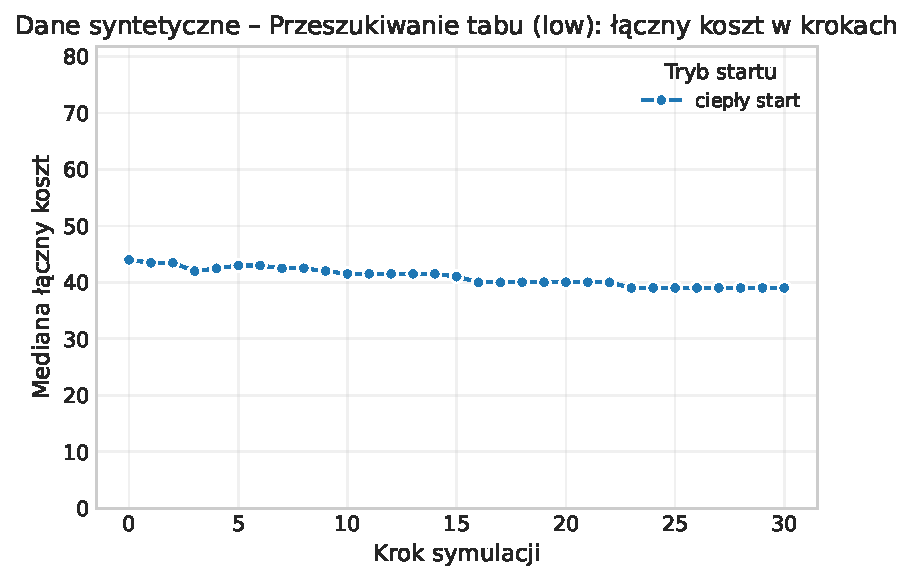
\includegraphics[width=0.62\linewidth]{assets/figures/dynamic/synthetic/synthetic_przeszukiwanie_tabu_cost_over_steps_low.pdf}\\[0.4em]
  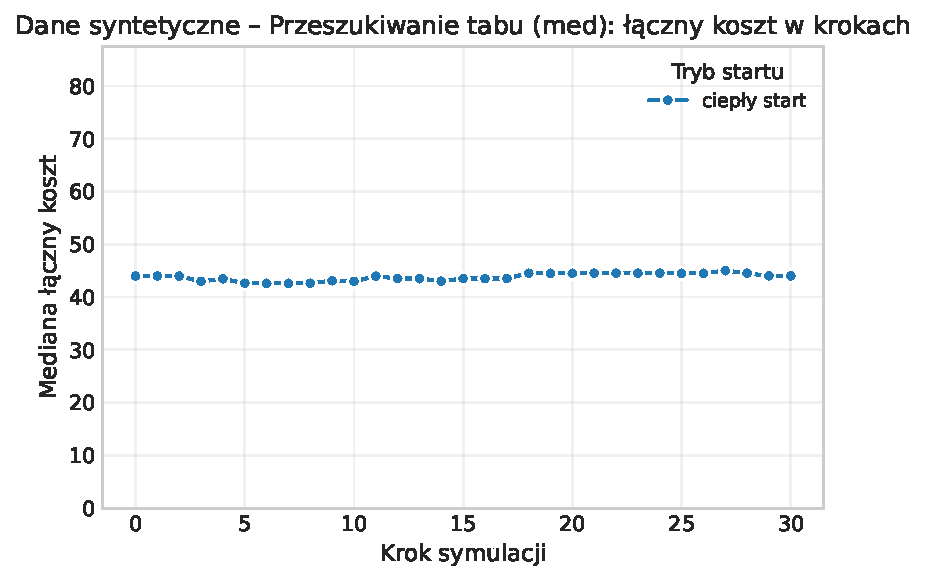
\includegraphics[width=0.62\linewidth]{assets/figures/dynamic/synthetic/synthetic_przeszukiwanie_tabu_cost_over_steps_med.pdf}\\[0.4em]
  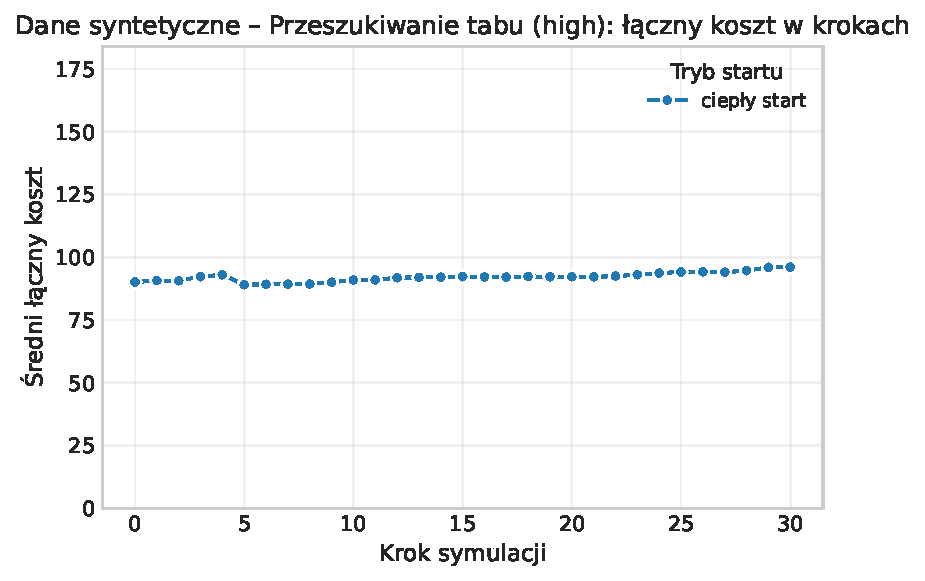
\includegraphics[width=0.62\linewidth]{assets/figures/dynamic/synthetic/synthetic_przeszukiwanie_tabu_cost_over_steps_high.pdf}
  \caption{Przeszukiwanie tabu -- koszt na węzeł w funkcji kroku (warianty low/med/high).}
  \label{fig:dyn-synth-tabu-cost}
\end{figure}

\begin{figure}[H]
  \centering
  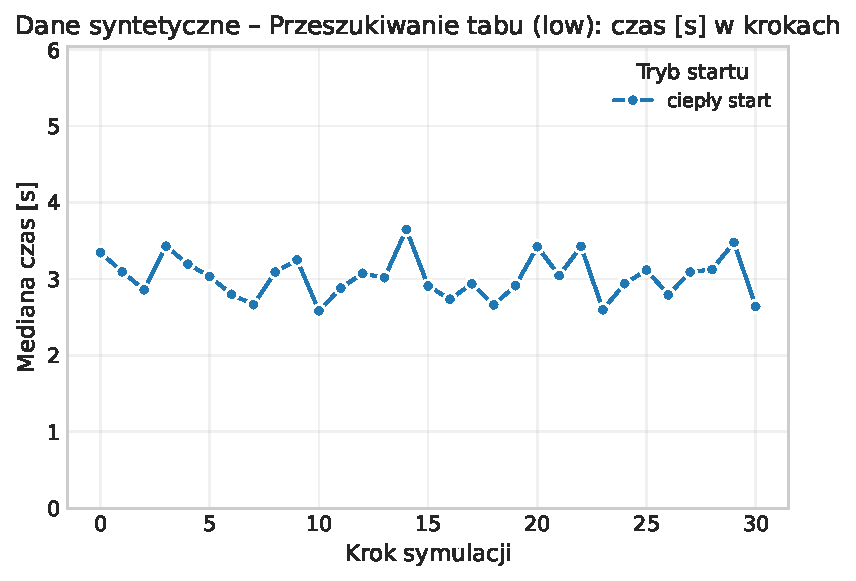
\includegraphics[width=0.62\linewidth]{assets/figures/dynamic/synthetic/synthetic_przeszukiwanie_tabu_time_over_steps_low.pdf}\\[0.4em]
  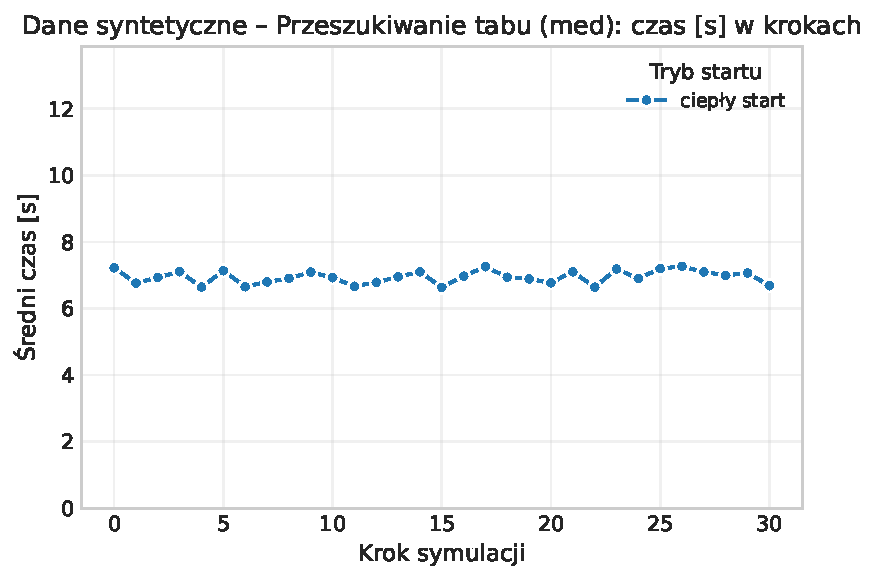
\includegraphics[width=0.62\linewidth]{assets/figures/dynamic/synthetic/synthetic_przeszukiwanie_tabu_time_over_steps_med.pdf}\\[0.4em]
  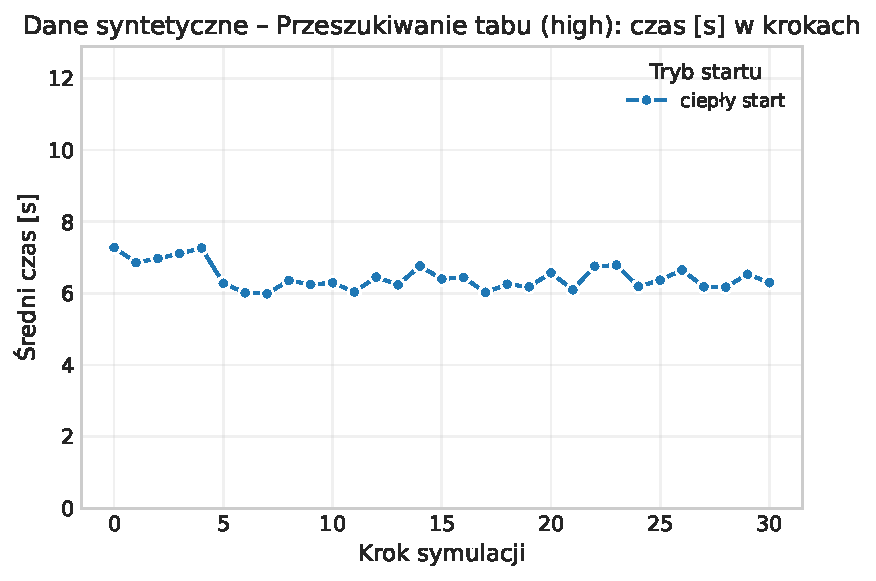
\includegraphics[width=0.62\linewidth]{assets/figures/dynamic/synthetic/synthetic_przeszukiwanie_tabu_time_over_steps_high.pdf}
  \caption{Przeszukiwanie tabu -- czas wykonania w funkcji kroku (warianty low/med/high).}
  \label{fig:dyn-synth-tabu-time}
\end{figure}

\begin{figure}[H]
  \centering
  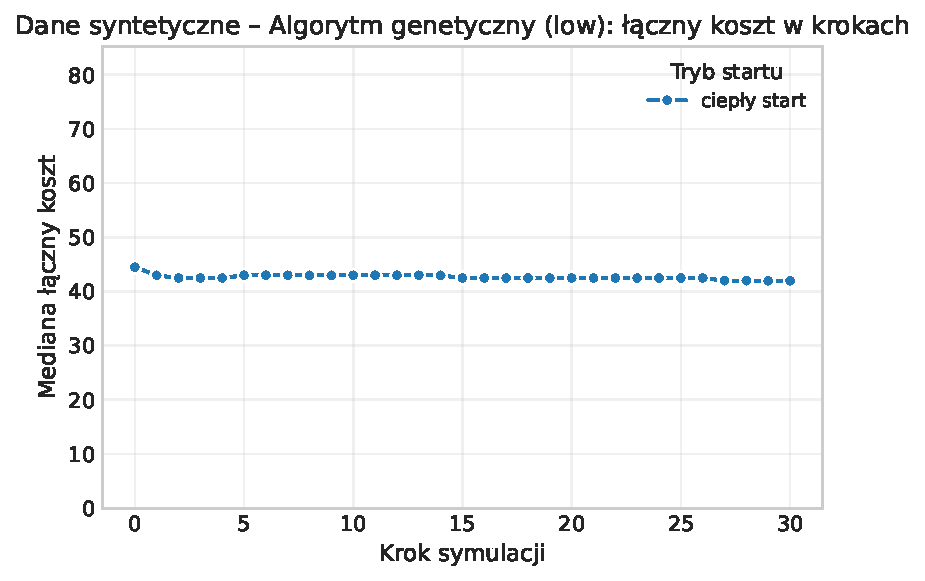
\includegraphics[width=0.62\linewidth]{assets/figures/dynamic/synthetic/synthetic_algorytm_genetyczny_cost_over_steps_low.pdf}\\[0.4em]
  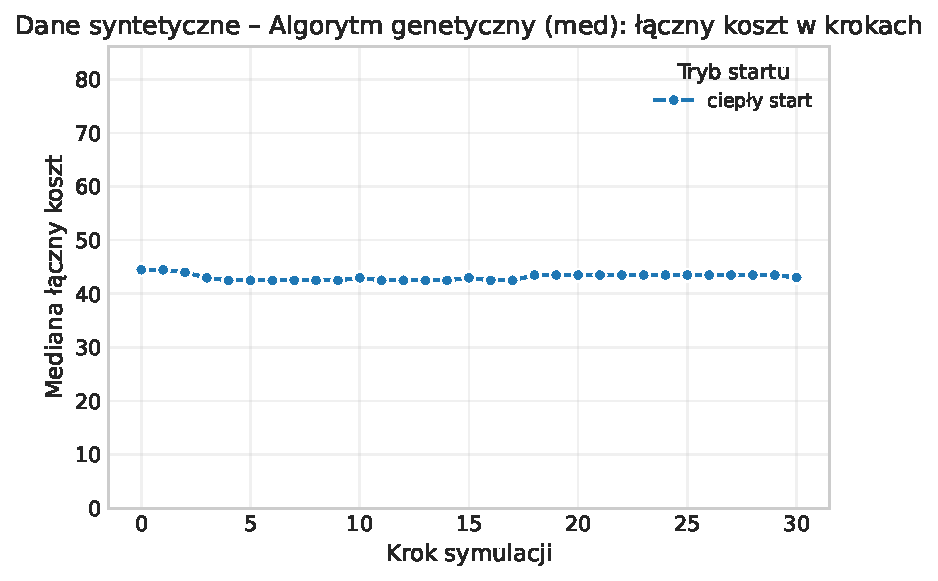
\includegraphics[width=0.62\linewidth]{assets/figures/dynamic/synthetic/synthetic_algorytm_genetyczny_cost_over_steps_med.pdf}\\[0.4em]
  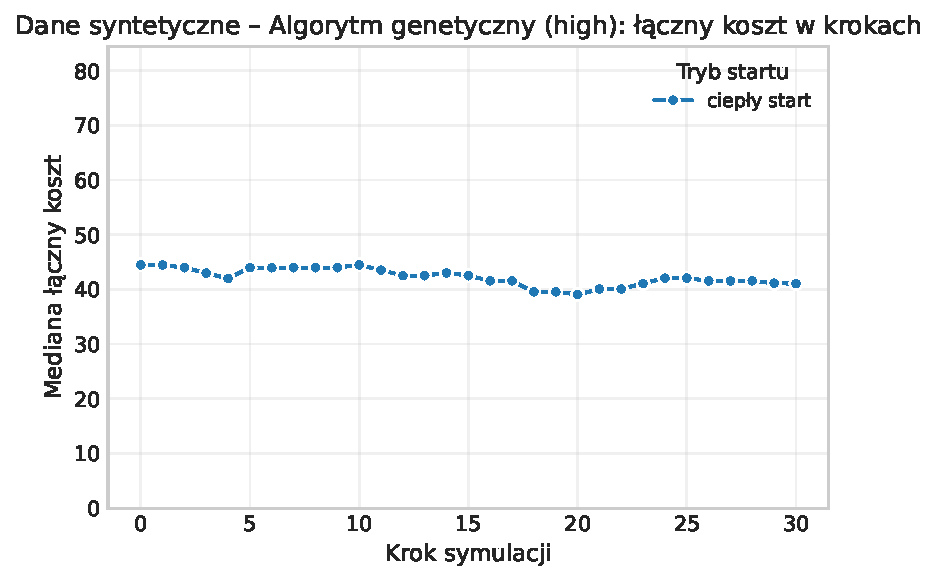
\includegraphics[width=0.62\linewidth]{assets/figures/dynamic/synthetic/synthetic_algorytm_genetyczny_cost_over_steps_high.pdf}
  \caption{Algorytm genetyczny -- koszt na węzeł w funkcji kroku (warianty low/med/high).}
  \label{fig:dyn-synth-genetic-cost}
\end{figure}

\begin{figure}[H]
  \centering
  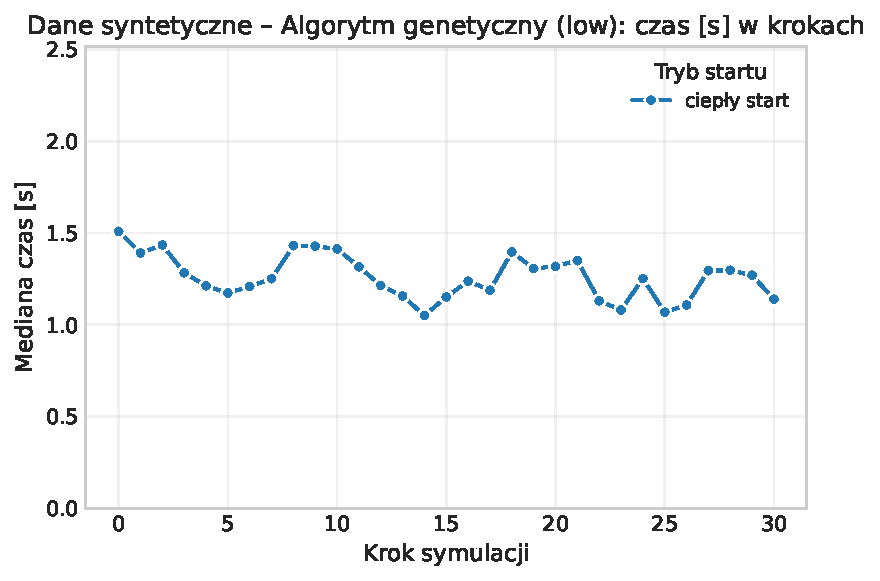
\includegraphics[width=0.62\linewidth]{assets/figures/dynamic/synthetic/synthetic_algorytm_genetyczny_time_over_steps_low.pdf}\\[0.4em]
  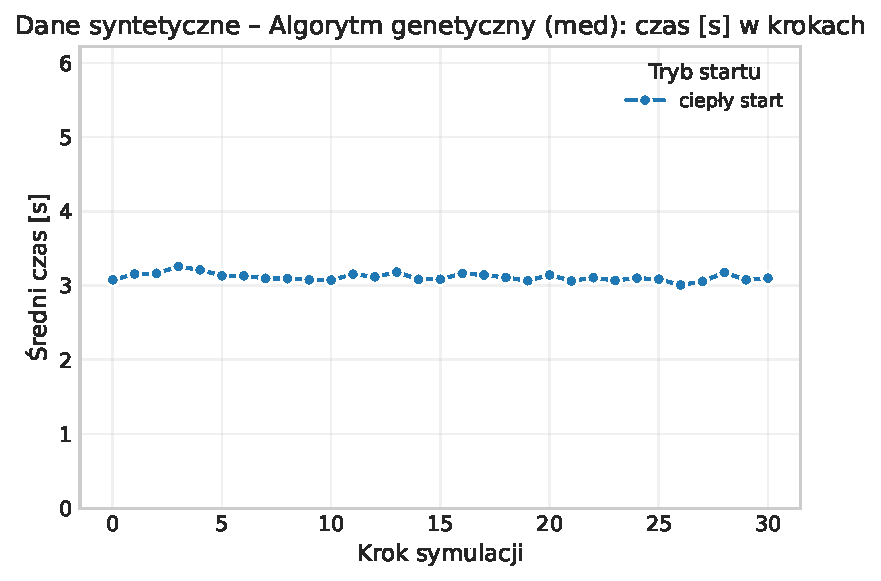
\includegraphics[width=0.62\linewidth]{assets/figures/dynamic/synthetic/synthetic_algorytm_genetyczny_time_over_steps_med.pdf}\\[0.4em]
  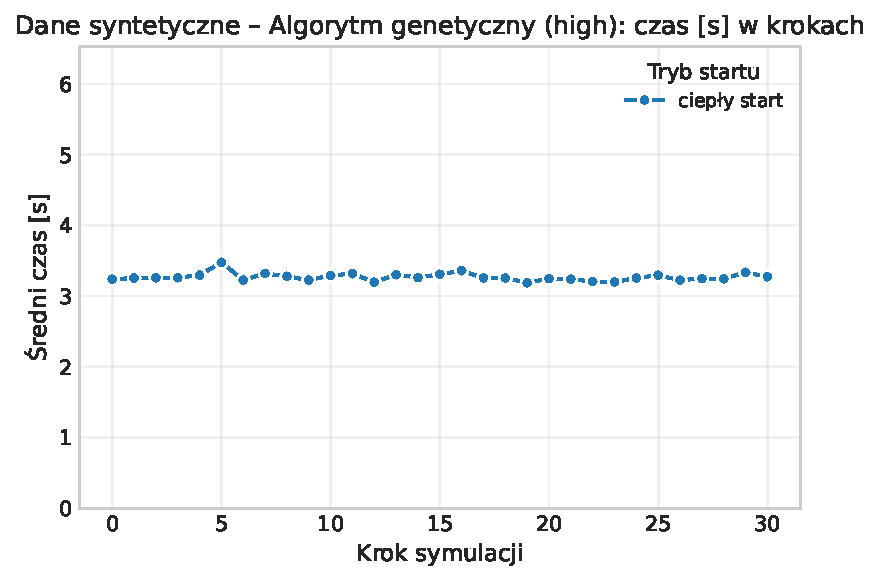
\includegraphics[width=0.62\linewidth]{assets/figures/dynamic/synthetic/synthetic_algorytm_genetyczny_time_over_steps_high.pdf}
  \caption{Algorytm genetyczny -- czas wykonania w funkcji kroku (warianty low/med/high).}
  \label{fig:dyn-synth-genetic-time}
\end{figure}

\begin{figure}[H]
  \centering
  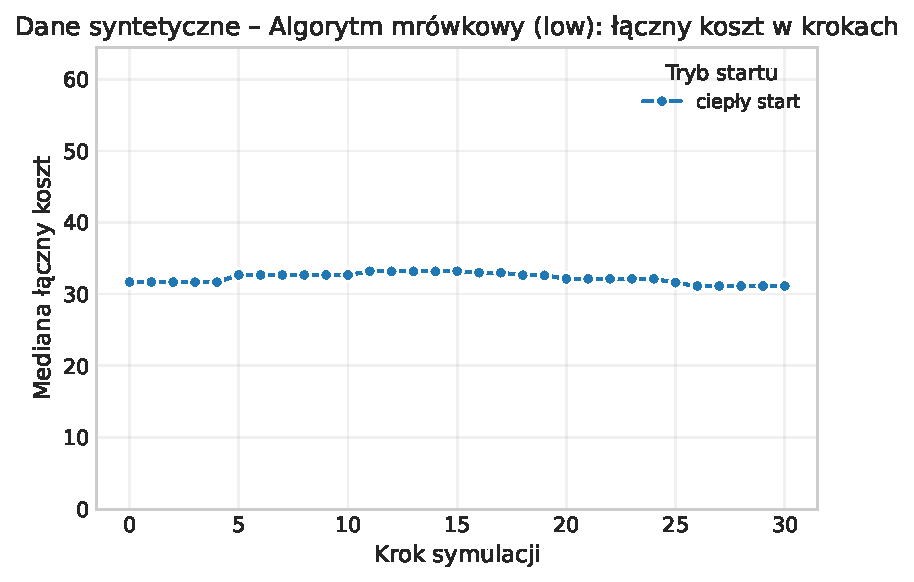
\includegraphics[width=0.62\linewidth]{assets/figures/dynamic/synthetic/synthetic_algorytm_mrowkowy_cost_over_steps_low.pdf}\\[0.4em]
  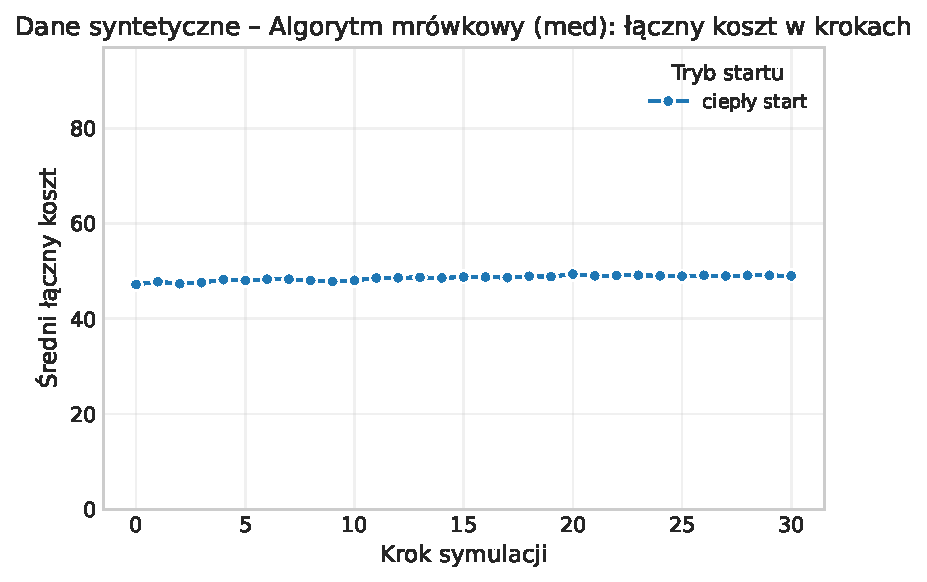
\includegraphics[width=0.62\linewidth]{assets/figures/dynamic/synthetic/synthetic_algorytm_mrowkowy_cost_over_steps_med.pdf}\\[0.4em]
  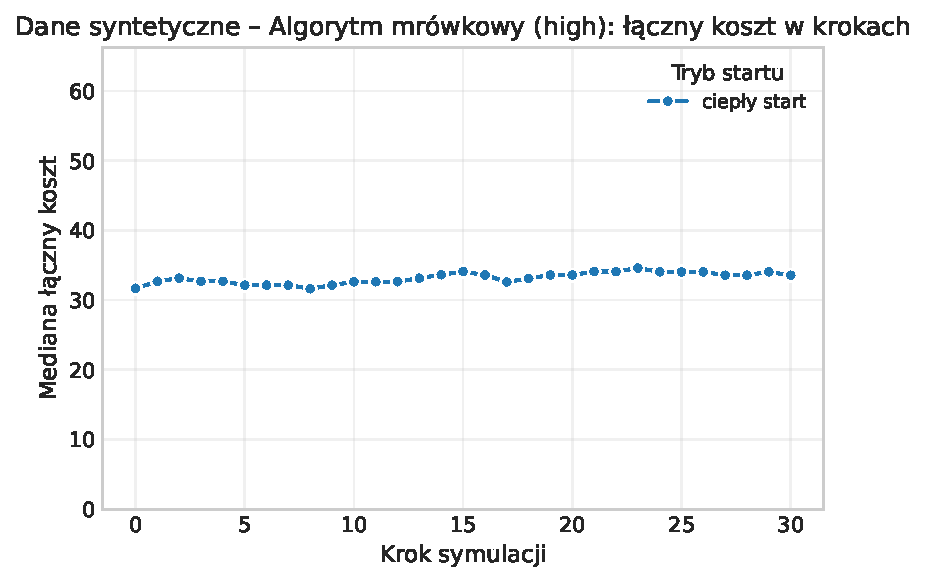
\includegraphics[width=0.62\linewidth]{assets/figures/dynamic/synthetic/synthetic_algorytm_mrowkowy_cost_over_steps_high.pdf}
  \caption{Algorytm mrówkowy -- koszt na węzeł w funkcji kroku (warianty low/med/high).}
  \label{fig:dyn-synth-aco-cost}
\end{figure}

\begin{figure}[H]
  \centering
  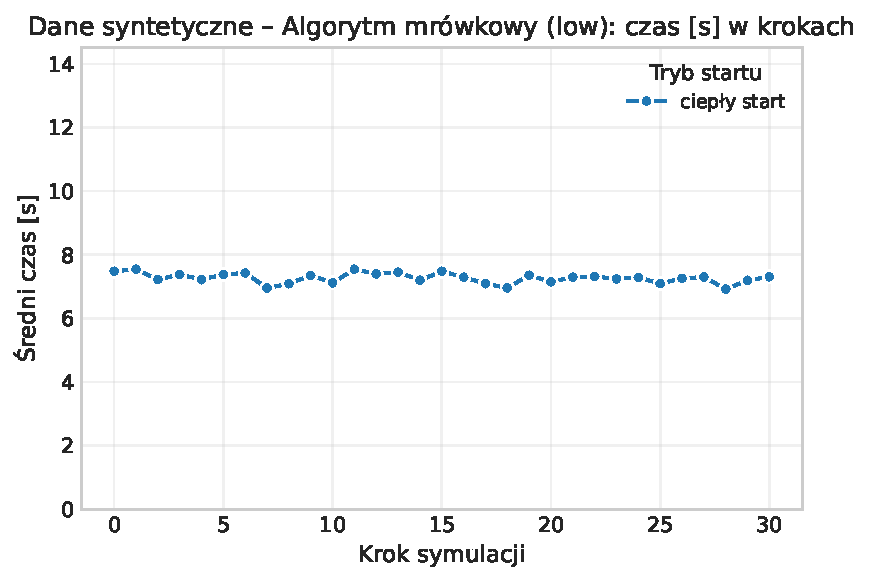
\includegraphics[width=0.62\linewidth]{assets/figures/dynamic/synthetic/synthetic_algorytm_mrowkowy_time_over_steps_low.pdf}\\[0.4em]
  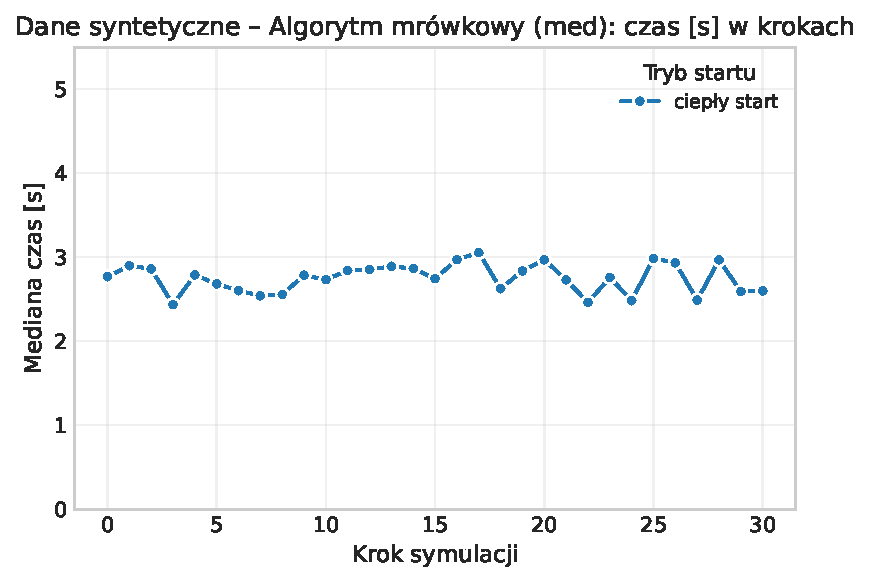
\includegraphics[width=0.62\linewidth]{assets/figures/dynamic/synthetic/synthetic_algorytm_mrowkowy_time_over_steps_med.pdf}\\[0.4em]
  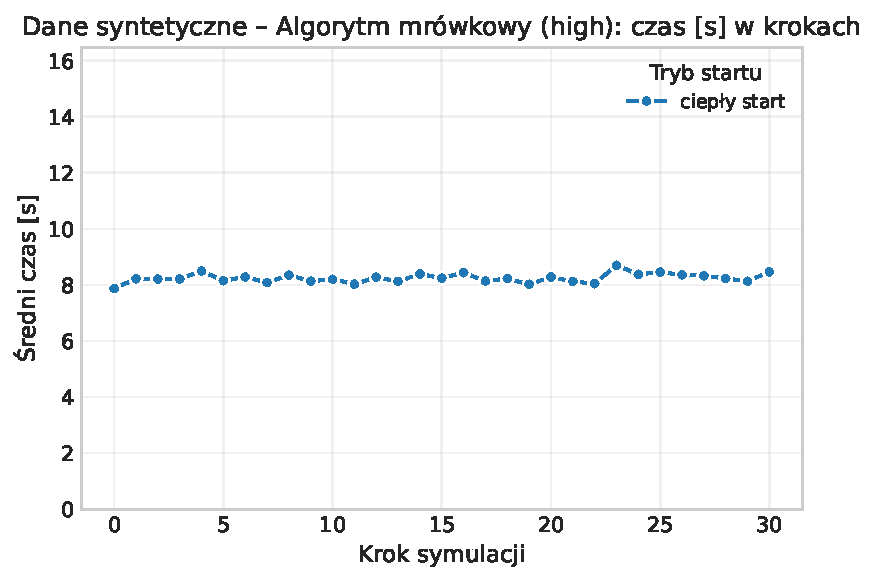
\includegraphics[width=0.62\linewidth]{assets/figures/dynamic/synthetic/synthetic_algorytm_mrowkowy_time_over_steps_high.pdf}
  \caption{Algorytm mrówkowy -- czas wykonania w funkcji kroku (warianty low/med/high).}
  \label{fig:dyn-synth-aco-time}
\end{figure}

\section{Wyniki realistyczne}

\subsection{Ciepły start metaheurystyk}

Tabela~\ref{tab:dyn-real-alg} prezentuje zbiorcze wyniki dla symulacji z preferencyjnym i triadycznym przyłączaniem. \textbf{Algorytm mrówkowy} pozostaje najtańszy jakościowo, ale \textbf{Przeszukiwanie tabu} oferuje porównywalny koszt przy najniższych medianach czasowych wśród metod wysokiej jakości (ok.~1.3~s).

\begin{table}[H]
  \centering
  \caption{Ciepły start (średnia po wariantach realistycznych).}
  \label{tab:dyn-real-alg}
  \begin{tabular}{lrrrrrr}
    \toprule
    \textbf{Algorytm}     & \textbf{Med. koszt} & \textbf{Śr. koszt} & \textbf{Med. koszt/węzeł} & \textbf{Śr. koszt/węzeł} & \textbf{Med. czas [s]} & \textbf{Śr. czas [s]} \\
    \midrule
    Algorytm genetyczny   & 54.83               & 89.51              & 0.397                     & 0.416                    & 0.502                  & 0.991                 \\
    Algorytm mrówkowy     & 52.50               & 83.60              & 0.418                     & 0.424                    & 1.891                  & 5.909                 \\
    Przeszukiwanie tabu   & 56.14               & 96.24              & 0.415                     & 0.426                    & 1.284                  & 2.175                 \\
    Wyżarzanie symulowane & 66.46               & 102.44             & 0.467                     & 0.473                    & 0.415                  & 0.884                 \\
  \end{tabular}
\end{table}

\subsection{Wpływ wariantu mutacji}

Mediany kosztu i czasu przeszukiwania tabu dla poszczególnych scenariuszy pokazano w tab.~\ref{tab:dyn-real-variants}. Wariant \texttt{pref\_triadic} generuje najtańsze rozwiązania dzięki wzmocnionej klastrowości, lecz jest tylko nieznacznie szybszy od \texttt{pref\_pref}. Dodanie losowego przełączania krawędzi (\texttt{rand\_rewire}) podnosi zarówno koszt, jak i czas rebalansowania.

\begin{table}[H]
  \centering
  \caption{Przeszukiwanie tabu -- mediany w zależności od scenariusza realistycznego.}
  \label{tab:dyn-real-variants}
  \begin{tabular}{lrr}
    \toprule
    \textbf{Wariant}       & \textbf{Med. koszt/węzeł} & \textbf{Med. czas [s]} \\
    \midrule
    \texttt{pref\_triadic} & 0.397                     & 1.194                  \\
    \texttt{pref\_pref}    & 0.416                     & 1.280                  \\
    \texttt{rand\_rewire}  & 0.431                     & 1.376                  \\
  \end{tabular}
\end{table}

Dodatkowa agregacja względem typu grafu (losowy, scale-free, małoświatowy) przedstawiona w tab.~\ref{tab:dyn-real-graph-type} potwierdza, że struktury scale-free są najkosztowniejsze, natomiast sieci małoświatowe pozostają najszybsze do obsługi.

\begin{table}[H]
  \centering
  \caption{Mediany kosztu na węzeł i czasu według typu grafu rzeczywistego.}
  \label{tab:dyn-real-graph-type}
  \begin{tabular}{lrr}
    \toprule
    \textbf{Typ grafu} & \textbf{Med. koszt/węzeł} & \textbf{Med. czas [s]} \\
    \midrule
    losowy             & 0.453                     & 0.205                  \\
    scale-free         & 0.686                     & 0.222                  \\
    małoświatowy       & 0.467                     & 0.193                  \\
  \end{tabular}
\end{table}

\subsection{Zimny start i benchmarki}

Zimny start dla scenariuszy realistycznych zestawiono w tab.~\ref{tab:dyn-real-cold}. Podobnie jak w przypadku danych syntetycznych, \textbf{Solver ILP} zapewnia najniższe koszty, ale wymaga rzędu 2~s na krok. \textbf{Algorytm zachłanny} i \textbf{Algorytm losowy} działają praktycznie natychmiast, pozostając użytecznymi baseline'ami.

\begin{table}[H]
  \centering
  \caption{Zimny start (średnia po wariantach realistycznych).}
  \label{tab:dyn-real-cold}
  \begin{tabular}{lrrrrrr}
    \toprule
    \textbf{Algorytm}  & \textbf{Med. koszt} & \textbf{Śr. koszt} & \textbf{Med. koszt/węzeł} & \textbf{Śr. koszt/węzeł} & \textbf{Med. czas [s]} & \textbf{Śr. czas [s]} \\
    \midrule
    Algorytm losowy    & 104.23              & 157.91             & 0.766                     & 0.763                    & 0.001                  & 0.001                 \\
    Algorytm zachłanny & 60.84               & 97.29              & 0.462                     & 0.469                    & 0.001                  & 0.001                 \\
    Solver ILP         & 30.57               & 60.22              & 0.343                     & 0.375                    & 0.790                  & 2.154                 \\
    Zbiór dominujący   & 56.50               & 94.41              & 0.458                     & 0.456                    & 0.003                  & 0.013                 \\
  \end{tabular}
\end{table}

Różnice pomiędzy metaheurystykami a algorytmem zachłannym z zimnego startu zebrano w tab.~\ref{tab:dyn-real-delta}. Przeszukiwanie tabu oraz algorytm mrówkowy poprawiają koszt na węzeł o 7--8\% kosztem dodatkowych 1.4--2.4~s. \textbf{Wyżarzanie symulowane} jest najszybsze, lecz nieznacznie przegrywa kosztowo z zachłannym.

\begin{table}[H]
  \centering
  \caption{Różnice względem algorytmu zachłannego (ciepły start, scenariusze realistyczne).}
  \label{tab:dyn-real-delta}
  \begin{tabular}{lrr}
    \toprule
    \textbf{Algorytm}     & \textbf{$\Delta$ koszt/węzeł} & \textbf{$\Delta$ czas [s]} \\
    \midrule
    Algorytm genetyczny   & $-0.055$ (–12.0\%)            & $+0.602$                   \\
    Algorytm mrówkowy     & $-0.038$ (–8.2\%)             & $+2.386$                   \\
    Przeszukiwanie tabu   & $-0.031$ (–6.7\%)             & $+1.376$                   \\
    Wyżarzanie symulowane & $+0.036$ (+7.8\%)             & $+0.474$                   \\
  \end{tabular}
\end{table}

\subsection{Ewolucja kosztów w czasie}

Rysunki~\ref{fig:dyn-real-tabu-cost} i~\ref{fig:dyn-real-tabu-time} prezentują przebieg kosztu i czasu przeszukiwania tabu w zależności od wariantu realistycznego. Łączenie preferencyjnego przyłączania z triadycznym domykaniem sprzyja utrzymaniu najniższych kosztów, natomiast wariant z losowym przełączaniem krawędzi prowadzi do wolniejszej stabilizacji.

Pełne przebiegi dla algorytmu genetycznego i mrówkowego pokazano na rys.~\ref{fig:dyn-real-genetic-cost}--\ref{fig:dyn-real-genetic-time} oraz rys.~\ref{fig:dyn-real-aco-cost}--\ref{fig:dyn-real-aco-time}.

\begin{figure}[H]
  \centering
  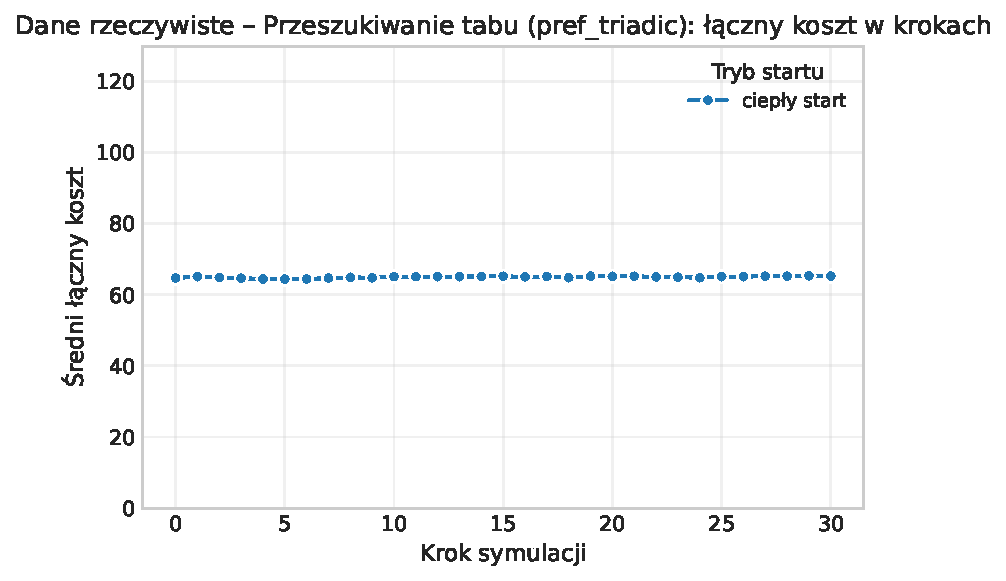
\includegraphics[width=0.62\linewidth]{assets/figures/dynamic/real/real_przeszukiwanie_tabu_cost_over_steps_pref_triadic.pdf}\\[0.4em]
  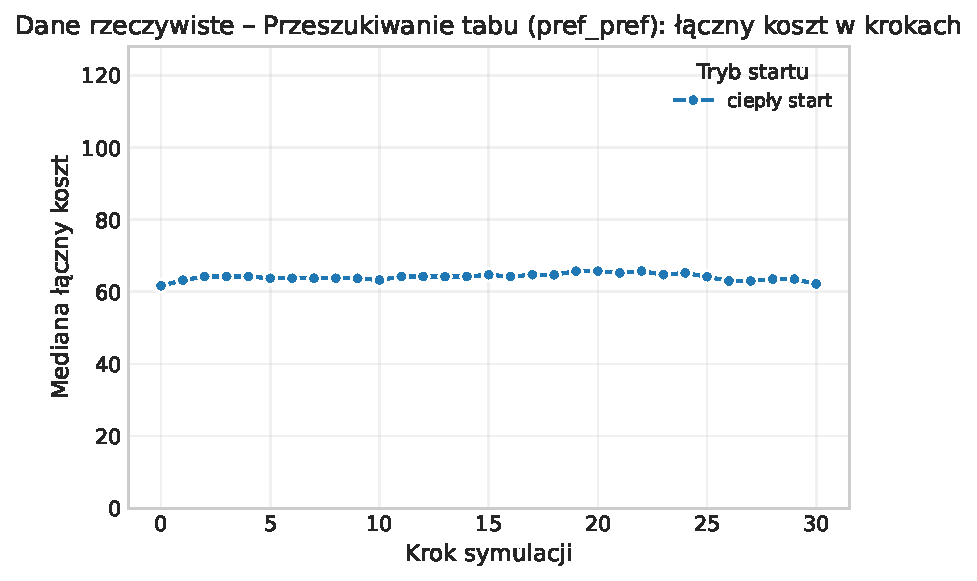
\includegraphics[width=0.62\linewidth]{assets/figures/dynamic/real/real_przeszukiwanie_tabu_cost_over_steps_pref_pref.pdf}\\[0.4em]
  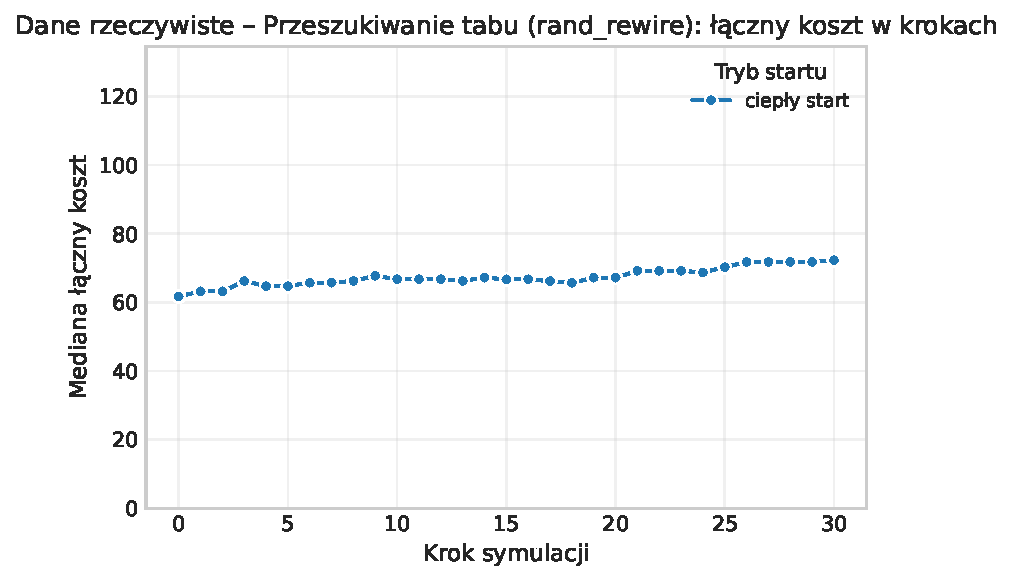
\includegraphics[width=0.62\linewidth]{assets/figures/dynamic/real/real_przeszukiwanie_tabu_cost_over_steps_rand_rewire.pdf}
  \caption{Przeszukiwanie tabu -- koszt na węzeł w scenariuszach realistycznych.}
  \label{fig:dyn-real-tabu-cost}
\end{figure}

\begin{figure}[H]
  \centering
  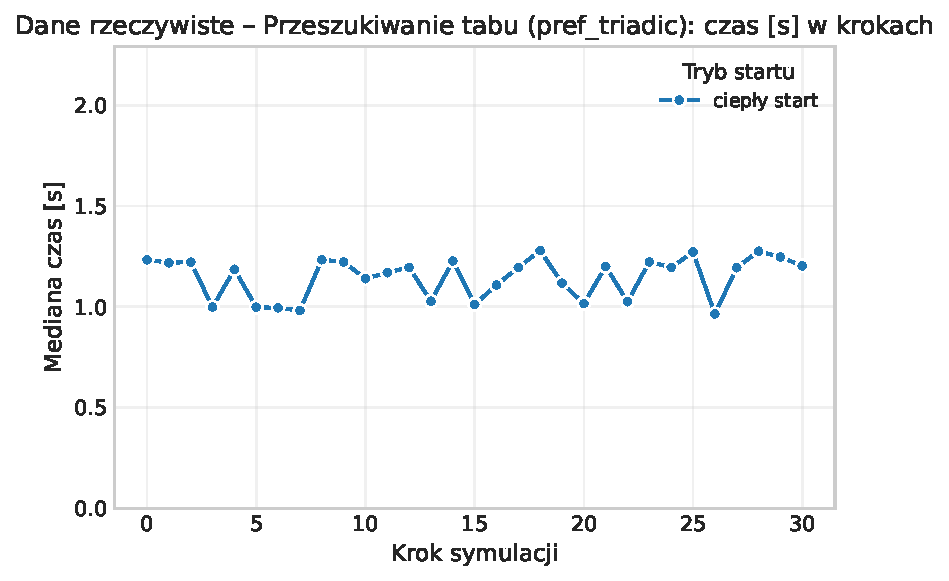
\includegraphics[width=0.62\linewidth]{assets/figures/dynamic/real/real_przeszukiwanie_tabu_time_over_steps_pref_triadic.pdf}\\[0.4em]
  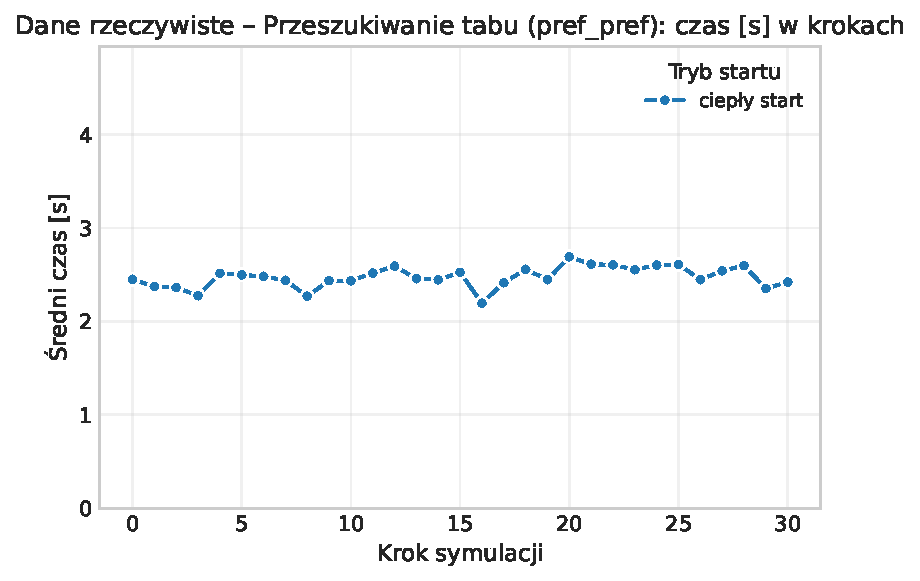
\includegraphics[width=0.62\linewidth]{assets/figures/dynamic/real/real_przeszukiwanie_tabu_time_over_steps_pref_pref.pdf}\\[0.4em]
  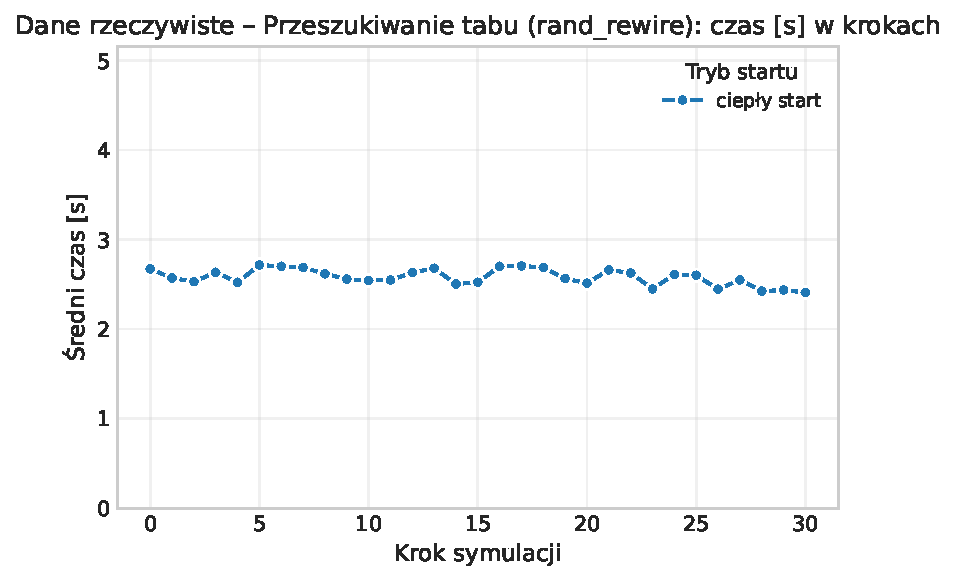
\includegraphics[width=0.62\linewidth]{assets/figures/dynamic/real/real_przeszukiwanie_tabu_time_over_steps_rand_rewire.pdf}
  \caption{Przeszukiwanie tabu -- czas wykonania w scenariuszach realistycznych.}
  \label{fig:dyn-real-tabu-time}
\end{figure}

\begin{figure}[H]
  \centering
  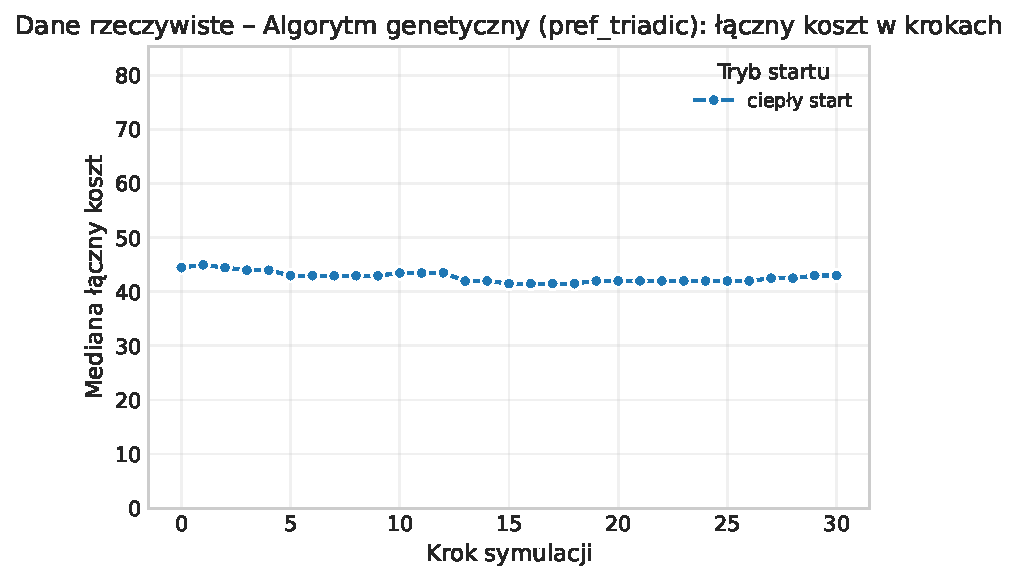
\includegraphics[width=0.62\linewidth]{assets/figures/dynamic/real/real_algorytm_genetyczny_cost_over_steps_pref_triadic.pdf}\\[0.4em]
  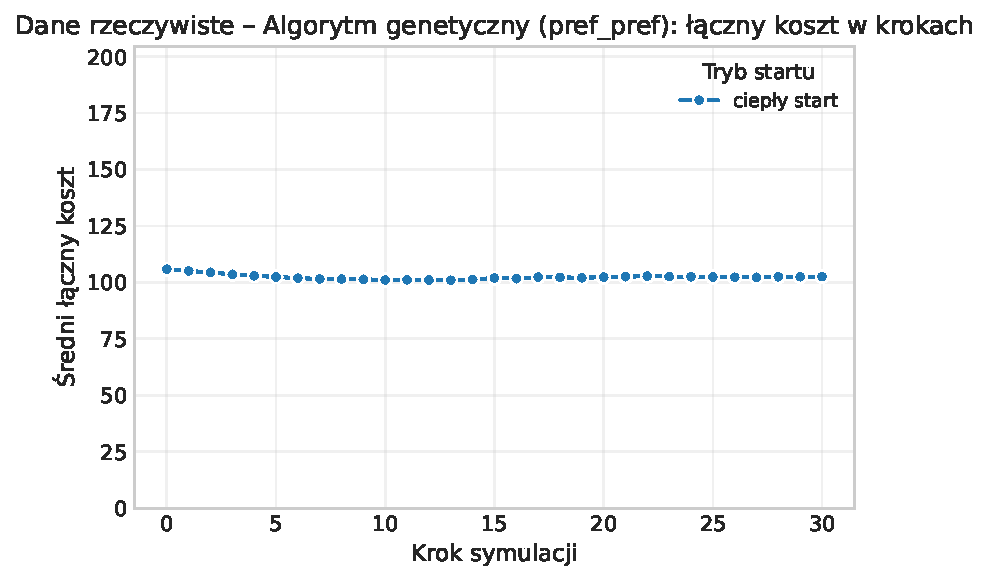
\includegraphics[width=0.62\linewidth]{assets/figures/dynamic/real/real_algorytm_genetyczny_cost_over_steps_pref_pref.pdf}\\[0.4em]
  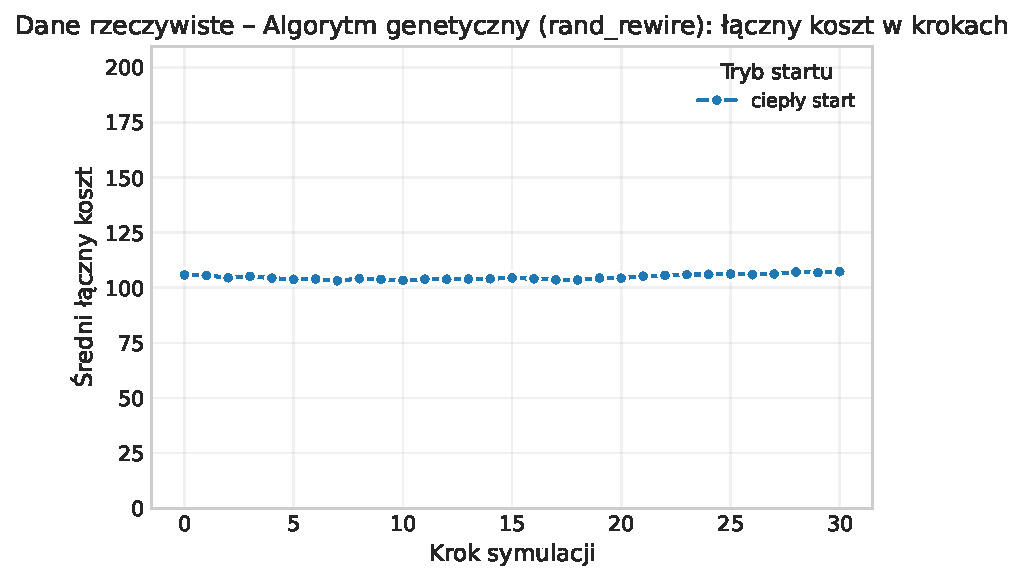
\includegraphics[width=0.62\linewidth]{assets/figures/dynamic/real/real_algorytm_genetyczny_cost_over_steps_rand_rewire.pdf}
  \caption{Algorytm genetyczny -- koszt na węzeł w wariantach realistycznych.}
  \label{fig:dyn-real-genetic-cost}
\end{figure}

\begin{figure}[H]
  \centering
  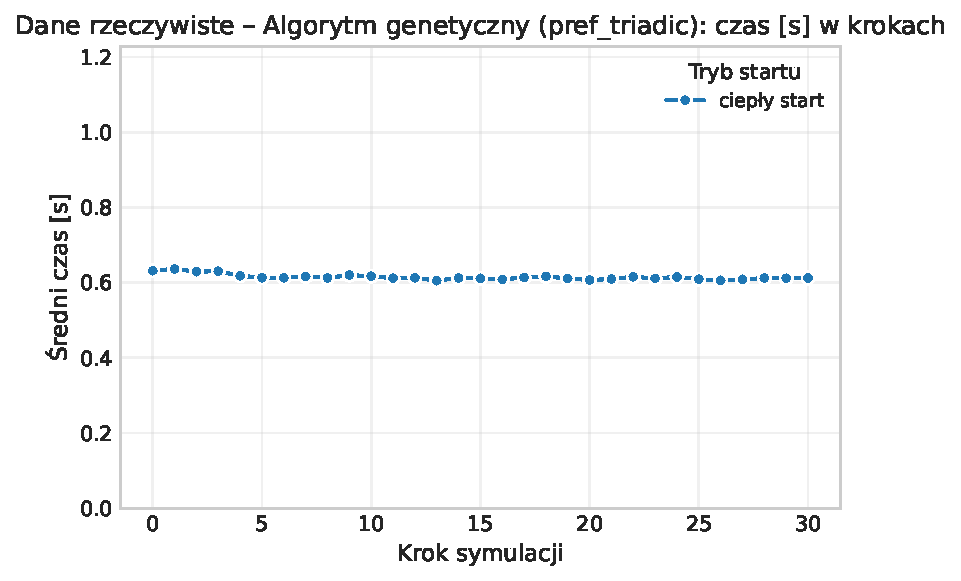
\includegraphics[width=0.62\linewidth]{assets/figures/dynamic/real/real_algorytm_genetyczny_time_over_steps_pref_triadic.pdf}\\[0.4em]
  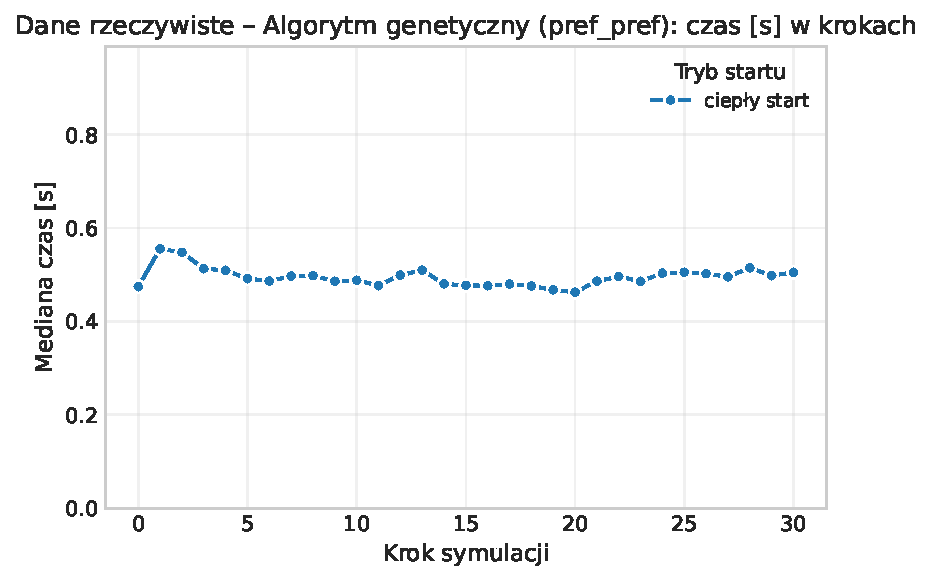
\includegraphics[width=0.62\linewidth]{assets/figures/dynamic/real/real_algorytm_genetyczny_time_over_steps_pref_pref.pdf}\\[0.4em]
  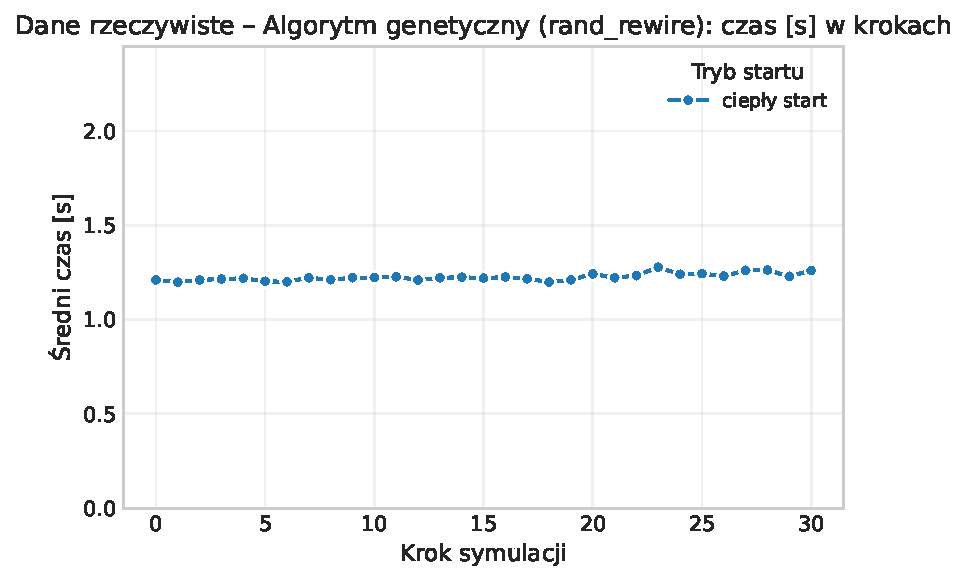
\includegraphics[width=0.62\linewidth]{assets/figures/dynamic/real/real_algorytm_genetyczny_time_over_steps_rand_rewire.pdf}
  \caption{Algorytm genetyczny -- czas wykonania w wariantach realistycznych.}
  \label{fig:dyn-real-genetic-time}
\end{figure}

\begin{figure}[H]
  \centering
  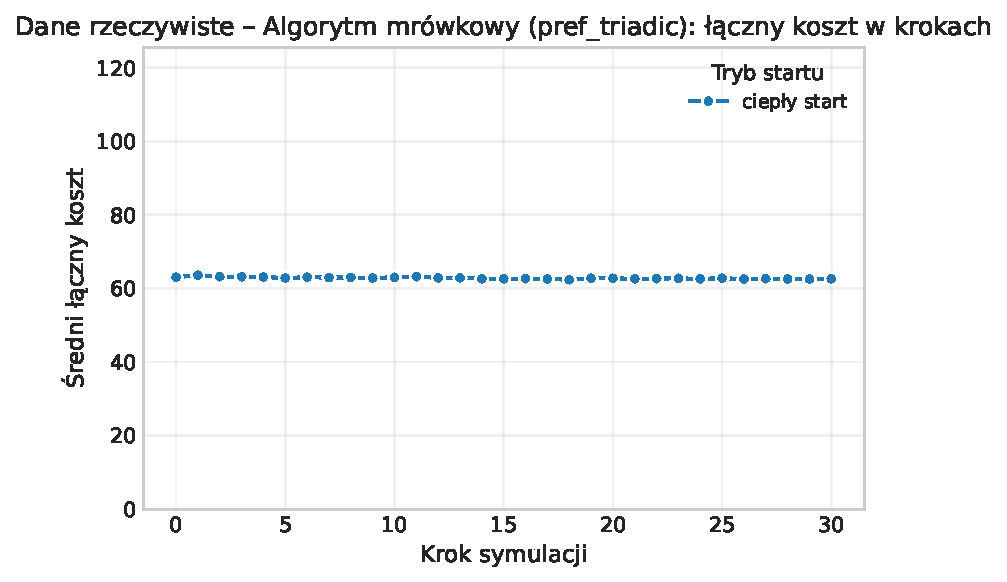
\includegraphics[width=0.62\linewidth]{assets/figures/dynamic/real/real_algorytm_mrowkowy_cost_over_steps_pref_triadic.pdf}\\[0.4em]
  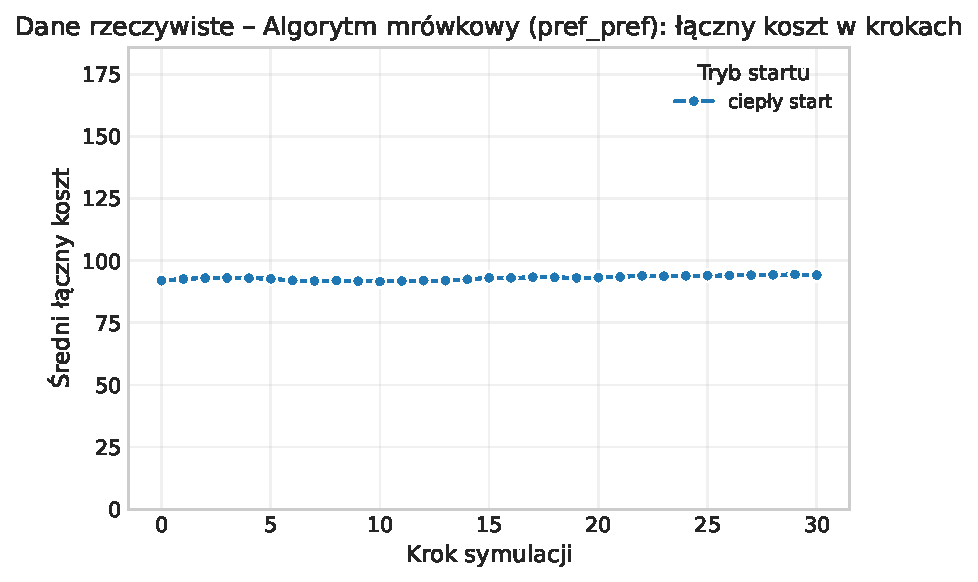
\includegraphics[width=0.62\linewidth]{assets/figures/dynamic/real/real_algorytm_mrowkowy_cost_over_steps_pref_pref.pdf}\\[0.4em]
  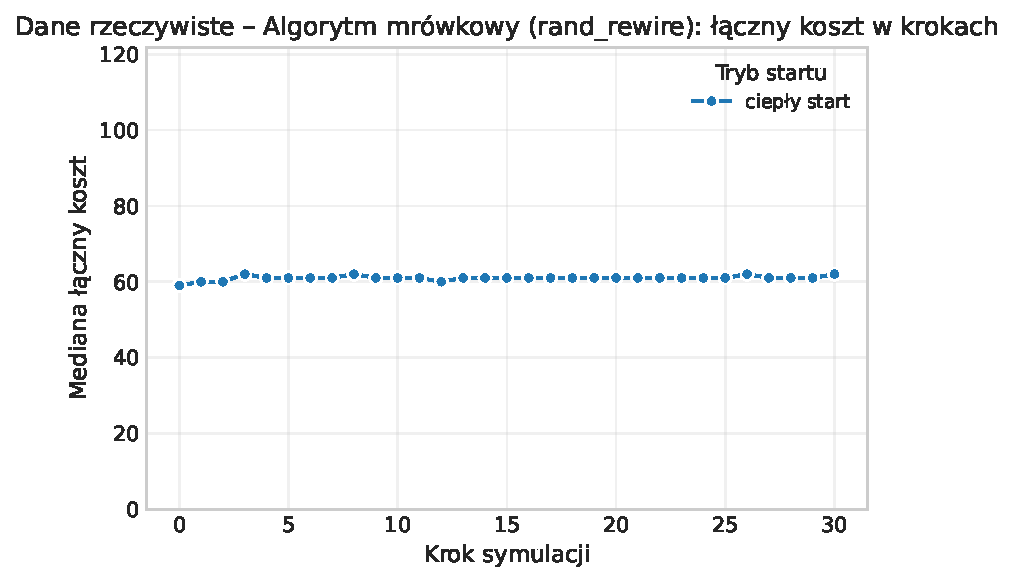
\includegraphics[width=0.62\linewidth]{assets/figures/dynamic/real/real_algorytm_mrowkowy_cost_over_steps_rand_rewire.pdf}
  \caption{Algorytm mrówkowy -- koszt na węzeł w wariantach realistycznych.}
  \label{fig:dyn-real-aco-cost}
\end{figure}

\begin{figure}[H]
  \centering
  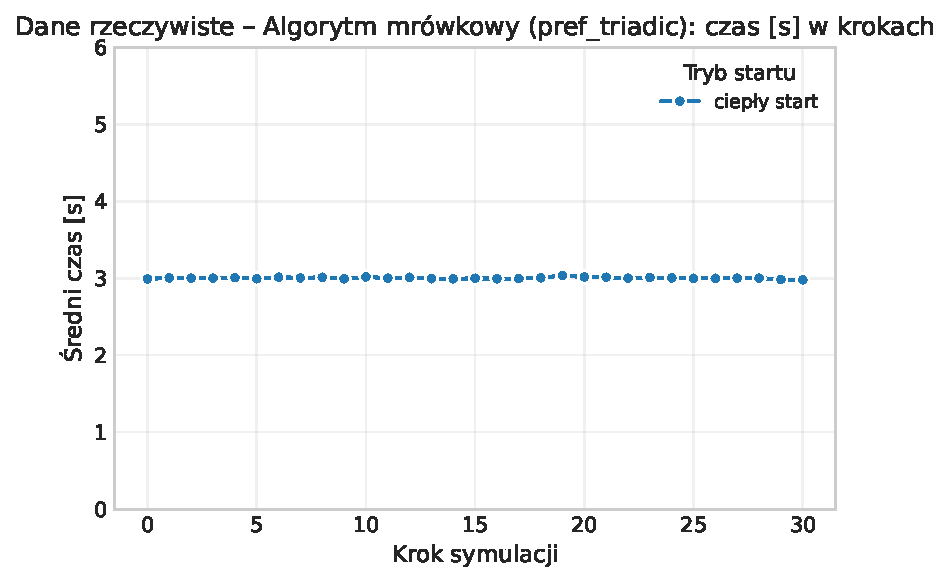
\includegraphics[width=0.62\linewidth]{assets/figures/dynamic/real/real_algorytm_mrowkowy_time_over_steps_pref_triadic.pdf}\\[0.4em]
  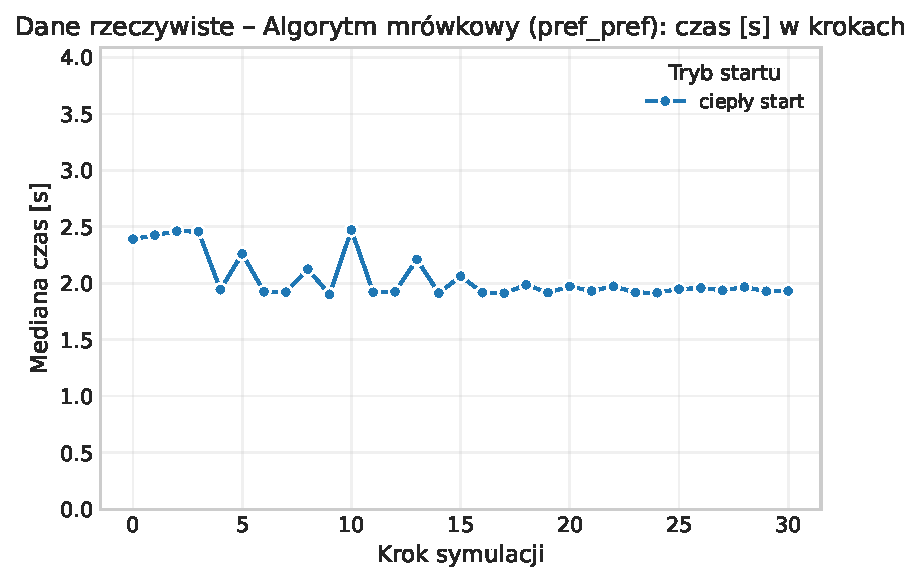
\includegraphics[width=0.62\linewidth]{assets/figures/dynamic/real/real_algorytm_mrowkowy_time_over_steps_pref_pref.pdf}\\[0.4em]
  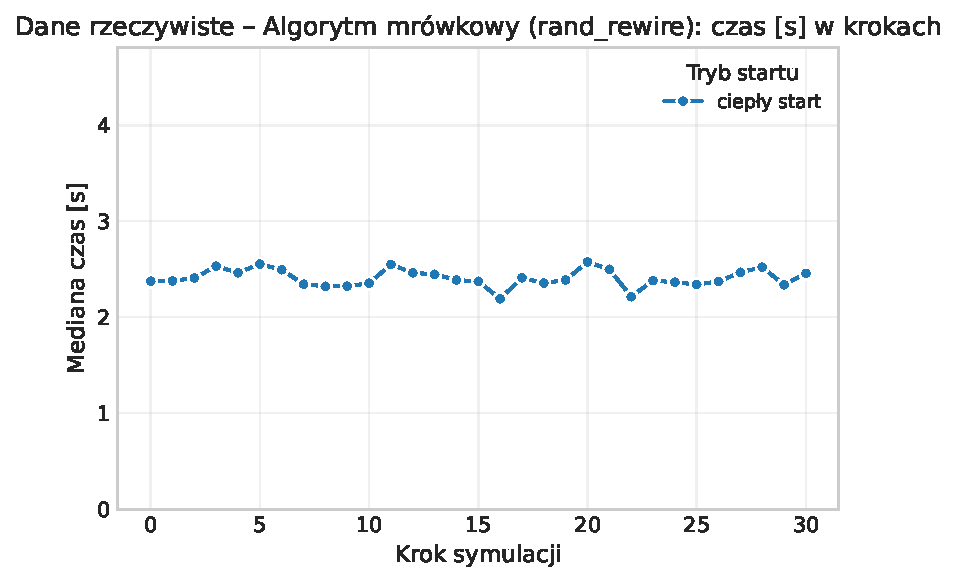
\includegraphics[width=0.62\linewidth]{assets/figures/dynamic/real/real_algorytm_mrowkowy_time_over_steps_rand_rewire.pdf}
  \caption{Algorytm mrówkowy -- czas wykonania w wariantach realistycznych.}
  \label{fig:dyn-real-aco-time}
\end{figure}

\section{Warm start kontra zimny start}

Zestawienie tabel \ref{tab:dyn-synth-warm}--\ref{tab:dyn-synth-delta} oraz \ref{tab:dyn-real-alg}--\ref{tab:dyn-real-delta} pokazuje, że wykorzystanie ciepłego startu pozwala metaheurystykom utrzymać koszt o 6--14\% niższy niż rozwiązanie zachłanne, zachowując akceptowalne czasy rzędu 1--3~s dla scenariuszy realistycznych i kilku sekund dla intensywnych mutacji syntetycznych. Mimo wzrostu czasów rebalansowania, ciepły start eliminuje konieczność pełnej rekalkulacji i umożliwia stabilne utrzymanie jakości rozwiązań w kolejnych krokach ewolucji sieci.
